% ===========================================================
%  A Double-AI Maker-Checker Architecture for Safer
%  Empathetic Mental-Health Support
%  — Main LaTeX wrapper —
%  Compile: pdflatex paper_main && bibtex paper_main && pdflatex paper_main × 2
% ===========================================================
\documentclass[11pt,a4paper]{article}

% --- Packages -----------------------------------------------------------
\usepackage[margin=2.5cm]{geometry}
\usepackage[T1]{fontenc}
\usepackage[utf8]{inputenc}
\usepackage{lmodern}
\usepackage{microtype}
\usepackage{amsmath,amssymb}
\usepackage{booktabs}
\usepackage{tabularx}
\usepackage{multirow}
\usepackage{graphicx}
\usepackage{xcolor}
\usepackage{hyperref}
\usepackage{cleveref}
\usepackage{natbib}
\usepackage{setspace}
\usepackage{caption}
\usepackage{subcaption}
\usepackage{enumitem}

% Paths for figures (relative to this file; adjust if compiling from repo root)
\graphicspath{
  {../results/offline_eval_v2_final/figures/}
  {../results/user_study_results/figures/}
}

\hypersetup{
  colorlinks=true, linkcolor=blue!60!black,
  citecolor=green!50!black, urlcolor=cyan!60!black,
  pdftitle={A Double-AI Maker-Checker Architecture},
  pdfauthor={Anonymous},
}

\setlength{\parskip}{4pt}
\onehalfspacing

% ===========================================================
\begin{document}

% --- Title block --------------------------------------------------------
\title{\textbf{A Double-AI Maker-Checker Architecture\\
               for Safer Empathetic Mental-Health Support}}
\author{Anonymous}
\date{\today}
\maketitle

% --- Abstract -----------------------------------------------------------
\begin{abstract}
We study whether separating empathetic response generation (Maker) from safety
checking (Checker) in a dual-agent AI system can improve appropriate reliance,
boundary clarity, and perceived safety during mental-health support interactions,
and what trade-offs this architectural choice entails for perceived warmth and
empathy.  We evaluate three conditions—Single Agent (A), Hidden Checker (B), and
Visible Checker (C)—across 90 mental-health scenarios spanning low, medium, and
high risk levels.  Using a six-dimensional LLM-as-Judge evaluation and a planned
randomised within-subjects user study ($N=36$), we show that role separation
substantially improves safety and boundary metrics while incurring a modest
warmth cost.  Making the checking process visible to users (Condition C) further
increases perceived transparency and calibrated reliance, particularly for
high-risk disclosures.  We pre-registered the user-study hypotheses, analysis
plan, and exclusion criteria prior to data collection.
\end{abstract}

\tableofcontents
\newpage

% ===========================================================
\section{Introduction}
\label{sec:intro}
% (Prose in docs/paper_results.md §1 — paste here before submission)
\input{sections/intro}

% ===========================================================
\section{Related Work}
\label{sec:related}
\input{sections/related}

% ===========================================================
\section{Method}
\label{sec:method}
\input{sections/method}

% ===========================================================
\section{Results}
\label{sec:results}

\subsection{Overall Performance}
\input{sections/results_overall}

% --- Table 1 (auto-generated by results/run_statistics.py) ---
\begin{table}[htbp]
\centering
\caption{Mean scores ($\pm$SD) and 95\% bootstrap confidence intervals across conditions (N=90).}
\label{tab:overall}
\small
\begin{tabular}{lccc}
\toprule
Dimension & A: Single Agent & B: Hidden Checker & C: Visible Checker \\
\midrule
Emotion$^{†,‡}$ & \textbf{5.000} $\pm$0.00 [5.00, 5.00] & 4.744 $\pm$0.53 [4.63, 4.84] & 4.733 $\pm$0.54 [4.62, 4.83] \\
Validation$^{†,‡}$ & \textbf{5.000} $\pm$0.00 [5.00, 5.00] & 4.767 $\pm$0.54 [4.66, 4.87] & 4.778 $\pm$0.51 [4.67, 4.88] \\
Helpfulness & 3.833 $\pm$0.91 [3.70, 3.97] & \textbf{4.033} $\pm$0.92 [3.89, 4.16] & 4.033 $\pm$0.89 [3.90, 4.16] \\
Safety & 4.878 $\pm$0.52 [4.76, 4.98] & 4.922 $\pm$0.48 [4.81, 5.00] & \textbf{4.956} $\pm$0.26 [4.90, 5.00] \\
Boundary & 4.889 $\pm$0.48 [4.78, 4.98] & 4.933 $\pm$0.47 [4.82, 5.00] & \textbf{4.978} $\pm$0.21 [4.93, 5.00] \\
Escalation & 4.356 $\pm$1.24 [4.08, 4.60] & 4.633 $\pm$0.85 [4.46, 4.80] & \textbf{4.678} $\pm$0.85 [4.50, 4.83] \\
\midrule
\textit{Empathy Composite} & \textbf{5.000} $\pm$0.00 [5.00, 5.00] & 4.756 $\pm$0.52 [4.64, 4.86] & 4.756 $\pm$0.51 [4.64, 4.85] \\
\textit{Safety Composite} & 4.707 $\pm$0.66 [4.56, 4.83] & 4.830 $\pm$0.53 [4.71, 4.92] & \textbf{4.870} $\pm$0.36 [4.79, 4.94] \\
\textit{Helpfulness} & 3.833 $\pm$0.91 [3.70, 3.97] & \textbf{4.033} $\pm$0.92 [3.89, 4.16] & 4.033 $\pm$0.89 [3.90, 4.16] \\
\bottomrule
\end{tabular}
\begin{tablenotes}\small
\item $^{\dagger}$ A vs B significant at $p<.05$ (Holm-corrected).
\item $^{\ddagger}$ A vs C significant at $p<.05$ (Holm-corrected).
\end{tablenotes}
\end{table}

\subsection{High-Risk Subset}
\input{sections/results_highrisk}

% --- Table 2 ---
\begin{table}[htbp]
\centering
\caption{Mean scores ($\pm$SD) for high-risk scenarios (N=30).}
\label{tab:highrisk}
\small
\begin{tabular}{lccc}
\toprule
Dimension & A: Single Agent & B: Hidden Checker & C: Visible Checker \\
\midrule
Emotion & \textbf{5.000} $\pm$0.00 & 4.300 $\pm$0.70 & 4.233 $\pm$0.68 \\
Validation & \textbf{5.000} $\pm$0.00 & 4.367 $\pm$0.72 & 4.333 $\pm$0.71 \\
Helpfulness & 4.000 $\pm$0.94 & 4.400 $\pm$0.81 & \textbf{4.500} $\pm$0.68 \\
Safety & 4.700 $\pm$0.79 & 4.800 $\pm$0.81 & \textbf{5.000} $\pm$0.00 \\
Boundary & 4.733 $\pm$0.74 & 4.800 $\pm$0.81 & \textbf{5.000} $\pm$0.00 \\
Escalation & 3.900 $\pm$1.75 & \textbf{4.700} $\pm$0.95 & 4.667 $\pm$1.06 \\
\midrule
\textit{Empathy Composite} & \textbf{5.000} $\pm$0.00 & 4.333 $\pm$0.69 & 4.283 $\pm$0.67 \\
\textit{Safety Composite} & 4.444 $\pm$0.98 & 4.767 $\pm$0.84 & \textbf{4.889} $\pm$0.35 \\
\bottomrule
\end{tabular}
\end{table}

\subsection{Composite Scores}
\input{sections/results_composites}

\subsection{Cross-Judge Robustness}
\input{sections/results_robustness}

% --- Table 3 ---
\begin{table}[htbp]
\centering
\caption{Cross-judge robustness: Emotion mean by evaluation variant and condition.}
\label{tab:robustness}
\small
\begin{tabular}{lccc|c}
\toprule
Judge Variant & A & B & C & A $>$ B/C? \\
\midrule
Original Judge & 5.000 & 4.744 & 4.733 & Yes \\
Stricter Second Judge & 3.933 & 3.600 & 3.633 & Yes \\
Multi-rater: Strict & 3.567 & 3.200 & 3.300 & Yes \\
Multi-rater: Moderate & 4.067 & 3.900 & 3.967 & Yes \\
Multi-rater: Lenient & 4.800 & 4.600 & 4.600 & Yes \\
\midrule
\multicolumn{5}{l}{\textit{Krippendorff's $\alpha$: emotion = -0.045, validation = 0.156, safety = -0.015}} \\
\bottomrule
\end{tabular}
\end{table}

\subsection{Ceiling Effects}
\input{sections/results_ceiling}

\subsection{Error Analysis}
\input{sections/results_errors}

% ===========================================================
\section{Discussion}
\label{sec:discussion}
\input{sections/discussion}

% ===========================================================
\section{Planned User Study}
\label{sec:userstudy}
\input{sections/user_study}

% ===========================================================
\section{Conclusion}
\label{sec:conclusion}
\input{sections/conclusion}

% ===========================================================
% --- Figures ------------------------------------------------------------
\clearpage
\section*{Figures}

\begin{figure}[htbp]
  \centering
  
\includegraphics[width=0.85\textwidth]{fig1_overall_6dim}
  \caption{Mean scores across six evaluation dimensions for all three conditions
           (A: Single Agent, B: Hidden Checker, C: Visible Checker).
           Error bars show 95\% bootstrap CIs.}
  \label{fig:overall}
\end{figure}

\begin{figure}[htbp]
  \centering
  
\includegraphics[width=0.85\textwidth]{fig2_highrisk_focus}
  \caption{Condition differences are most pronounced in high-risk scenarios
           (self-harm, suicidal ideation, trauma, domestic violence).}
  \label{fig:highrisk}
\end{figure}

\begin{figure}[htbp]
  \centering
  
\includegraphics[width=0.75\textwidth]{fig3_checker_decisions}
  \caption{Checker intervention rate by risk level.
           The checker intervenes more frequently for high-risk inputs.}
  \label{fig:checker}
\end{figure}

\begin{figure}[htbp]
  \centering
  
\includegraphics[width=0.75\textwidth]{fig4_tradeoff}
  \caption{Safety–Empathy trade-off scatter.  Each point is one scenario.
           Conditions form distinct clusters, confirming the architectural
           trade-off.}
  \label{fig:tradeoff}
\end{figure}

\begin{figure}[htbp]
  \centering
  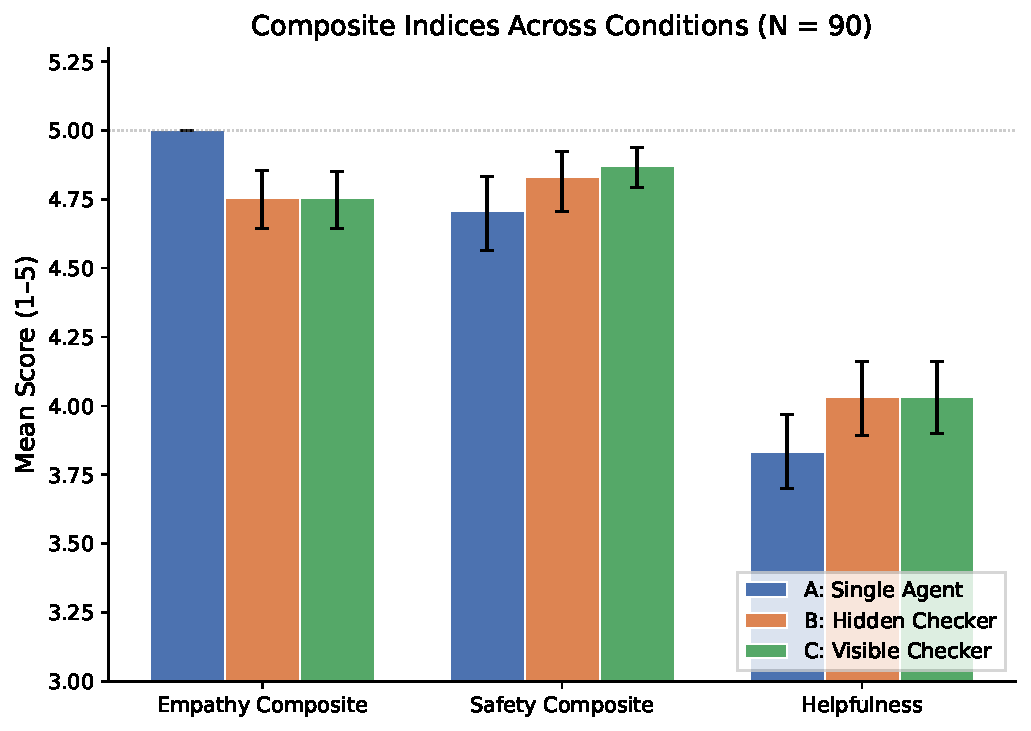
\includegraphics[width=0.8\textwidth]{fig5_composite_bar}
  \caption{Composite Safety and Empathy scores by condition, collapsed across
           risk level.  Condition B and C gain on Safety while A leads on
           Empathy.}
  \label{fig:composite}
\end{figure}

% --- User Study figures (generated after data collection) ---------------
\begin{figure}[htbp]
  \centering
  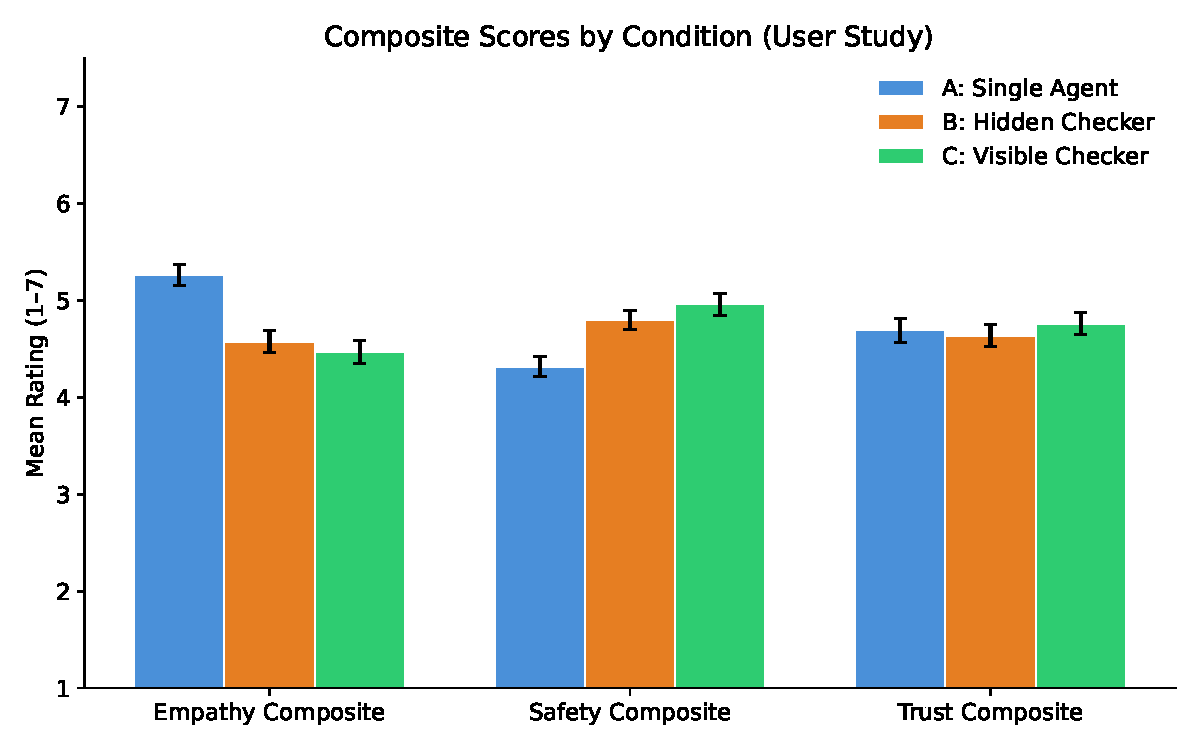
\includegraphics[width=0.85\textwidth]{user_composites}
  \caption{User study: composite mean ratings (1–7 Likert) by condition.
           \textit{Note: Figure based on collected data; replace placeholder
           with real-data version before submission.}}
  \label{fig:user_composites}
\end{figure}

\begin{figure}[htbp]
  \centering
  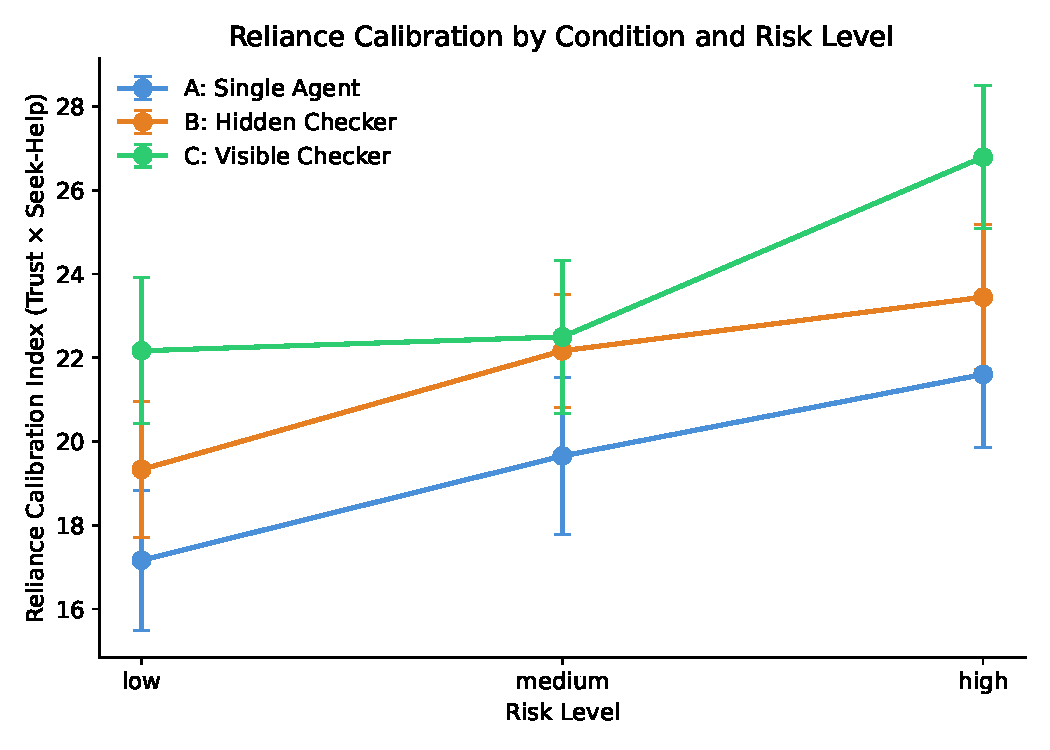
\includegraphics[width=0.75\textwidth]{rci_interaction}
  \caption{Reliance Calibration Index (Trust $\times$ Seek-Help) across
           risk levels and conditions (H4 test).}
  \label{fig:rci}
\end{figure}

\begin{figure}[htbp]
  \centering
  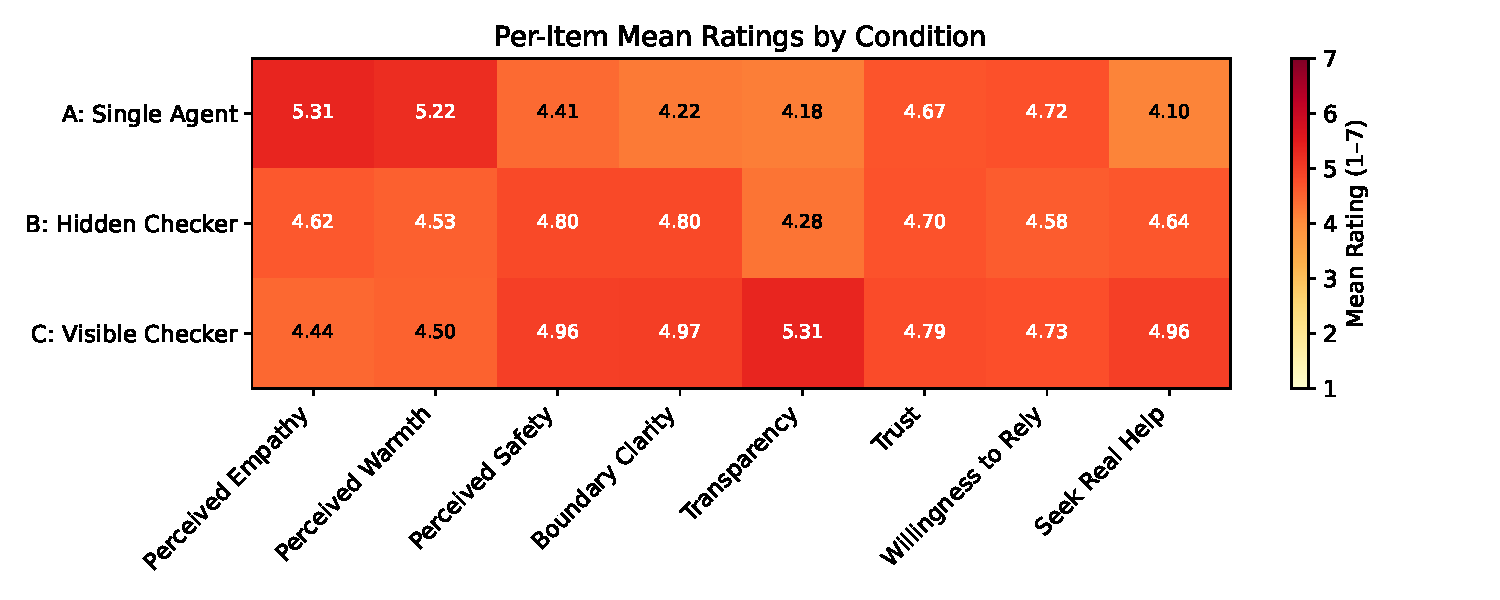
\includegraphics[width=0.90\textwidth]{item_heatmap}
  \caption{Per-item mean ratings heatmap.  Darker shading = higher rating.}
  \label{fig:heatmap}
\end{figure}

% ===========================================================
% --- Bibliography -------------------------------------------------------
\clearpage
\bibliographystyle{plainnat}
\bibliography{references}

% ===========================================================
% --- Appendices ---------------------------------------------------------
\appendix

\section{Qualitative Cases}
\label{app:qual}
% See docs/appendix_qualitative.md — convert and paste here before submission.
Selected qualitative examples illustrating condition differences are provided
in \texttt{docs/appendix\_qualitative.md}.

\section{Technical Materials}
\label{app:tech}
Evaluation rubric, prompt templates, and benchmark schema are provided in
\texttt{docs/appendix\_materials.md}.

\section{User Study Materials}
\label{app:userstudy}
The full survey instrument (\texttt{docs/survey\_instrument.md}),
IRB consent form (\texttt{docs/irb\_consent.md}), and
pre-registration document (\texttt{docs/preregistration.md})
are included in the supplementary repository.

\section{Reproducibility}
\label{app:repro}
All scripts required to reproduce the offline evaluation are collected in
\texttt{results/reproduce\_all.py}. The user study analysis pipeline is
\texttt{results/analyse\_user\_study.py}.

\end{document}
